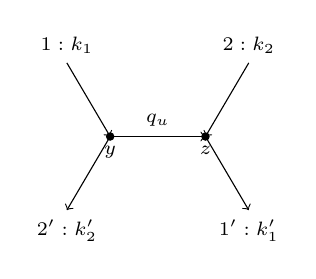
\begin{tikzpicture}[scale=1.1, every node/.style={font=\scriptsize}]
\coordinate (Y) at (-.55,0); \coordinate (Z) at (.55,0);
\draw[->] (-1.05,.85) node[above] {$1:k_1$} -- (Y);
\draw[->] (Y) -- (-1.05,-.85) node[below] {$2':k_2'$};
\draw[->] (1.05,.85) node[above] {$2:k_2$} -- (Z);
\draw[->] (Z) -- (1.05,-.85) node[below] {$1':k_1'$};
\draw[->] (Y) -- node[above] {$q_u$} (Z);
\fill (Y) circle (1.4pt) node[below] {$y$};
\fill (Z) circle (1.4pt) node[below] {$z$};
\end{tikzpicture}
